\vspace{-30pt}
\begin{figure}[h]
    \centering
    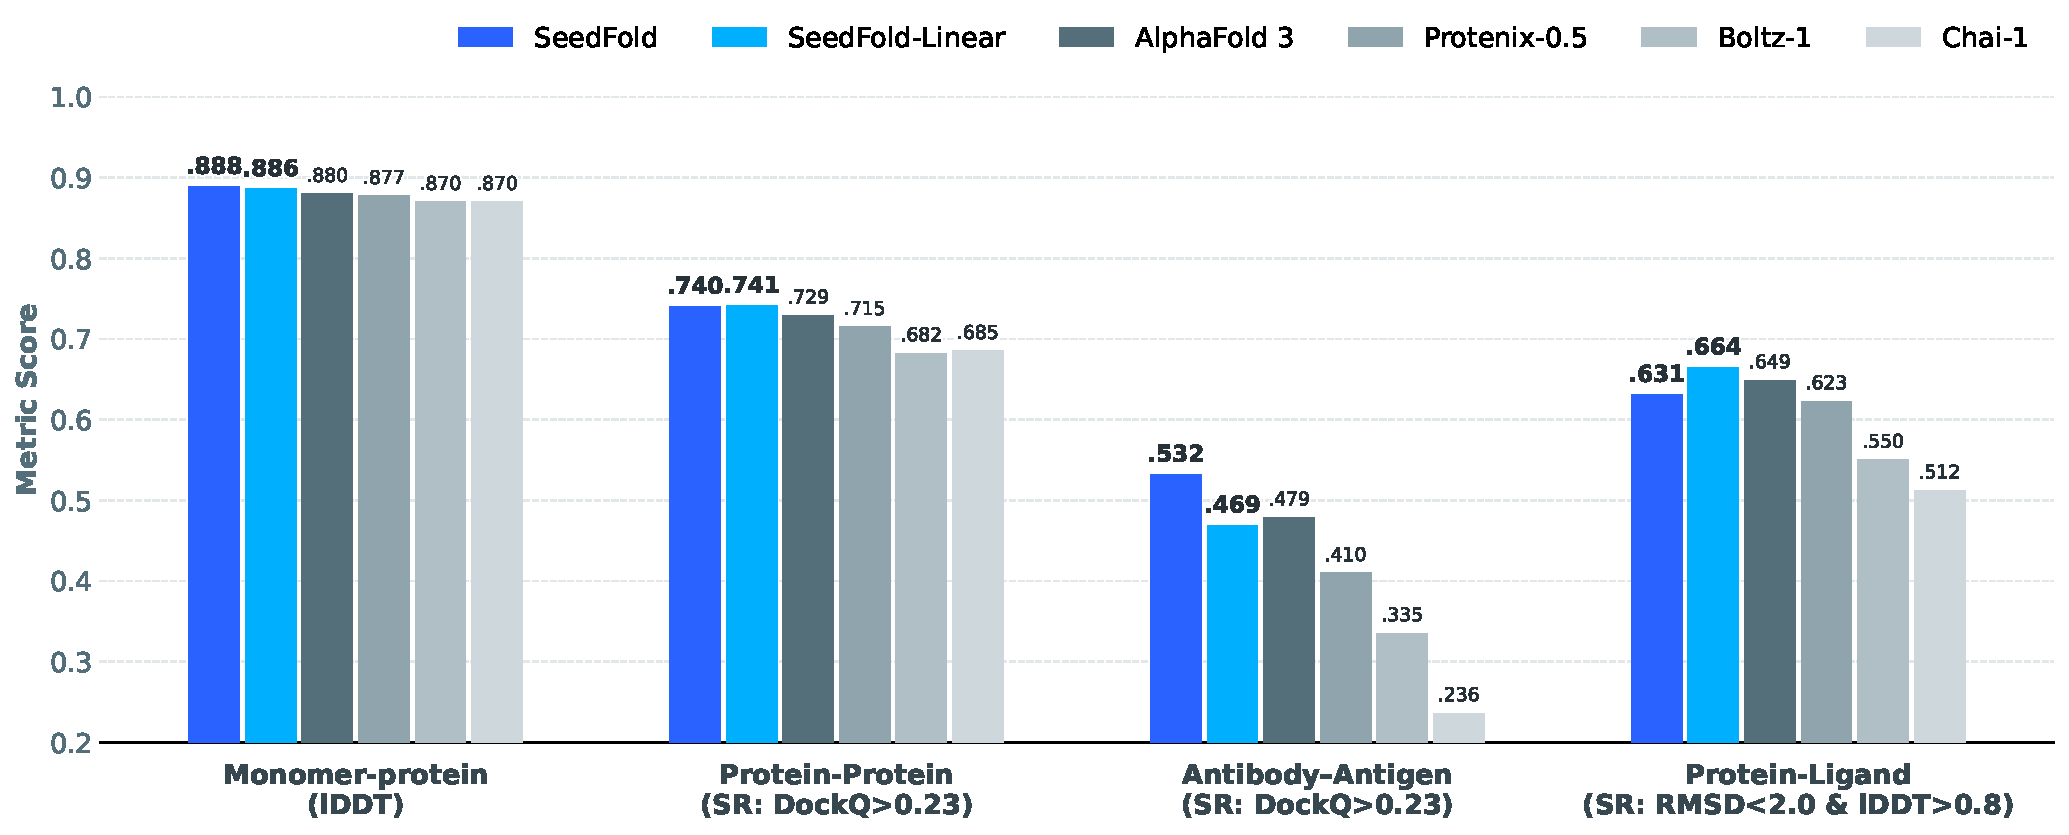
\includegraphics[width=0.95\linewidth]{figures/intro.pdf}
    \caption{Overview of \texttt{SeedFold}. (i) We scale folding models from three perspectives. \textbf{Model}: scaling the Pairformer width to increase model capacity; \textbf{Architecture}: linear triangular attention reduces computational complexity while maintaining prediction quality; \textbf{Data}: large-scale distillation expands training data to $26.5$M samples. (ii) \texttt{SeedFold} denotes a 512-width model equipped with vanilla triangular attention, while \texttt{SeedFold-Linear} refers to a 384-width model with linear attention. (iii) \texttt{SeedFold} achieves state-of-the-art performance on FoldBench, surpassing AlphaFold3 and other open-source models on multiple tasks. }
    \label{fig:front}
\end{figure}
% \todoq{add numbers on all the bars?}

% \todoq{Biomolecule Structure Prediction or Biomolecular Structure Prediction?}
\newpage
\section{Introduction}

% \todoq{perhaps use author year citation format, instead of number?}
Determining protein structures is crucial for structural biology and drug discovery. Experimental techniques, including X-ray crystallography and cryo-electron microscopy, facilitate the construction of high-resolution protein models; however, these approaches are considerably time-consuming. AlphaFold2~\cite{jumper2021highly} revolutionized protein structure prediction, achieving experimental-level accuracy for protein monomers in 2021. AlphaFold3~\cite{abramson2024accurate} further unifies the modeling of proteins, DNA, RNA, and ligands at an atomic level. There has been a line of research works~\cite{ahdritz2024openfold,wohlwend2025boltz,bytedance2025protenix,qiao2024neuralplexer3,chai2024chai,team2025intfold} focusing on high accuracy structure prediciton at AlphaFold-level, which has made a great contribution to the community. 

Folding models harness prior knowledge and exhibit versatility across an extensive spectrum of applications, including structure generation~\cite{watson2023novo,krishna2024generalized}, binder design~\cite{pacesa2024bindcraft}, conformation sampling~\cite{monteiro2024high}, or even in turn benefits experimental methods~\cite{raghu2025multiscaleguidanceproteinstructure,jamali2024automated}. Therefore, building effective folding models is a critical step towards creating protein foundation models. Modern foundation models such as GPT-4~\cite{abramson2024accurate} exhibit superior artificial general intelligence, yet their architectural design does not differ substantially from that of their predecessor, GPT-2, except for scaling the model size to an exponentially larger magnitude~\cite{radford2019language}. This raises two research questions: \textit{is current model capacity sufficient for protein structure modeling}, and \textit{what is the best way to scale these models}?

Although a few research works have attempted to examine the scaling behavior of such folding models~\cite{qiao2024neuralplexer3,passaro2025boltz}, most recent folding models adhere to the basic configurations of AlphaFold. They have mainly focused on scaling the number of Pairformer layers, while we find the performance of folding models may be bounded by the hidden dimension, which bottlenecks their capacity. The recycling strategy of AlphaFold (up to $3$ at the training stage and $9$ at the inference stage) has already approximated the increase in the model depth, which has proven better at representation learning than its non-recursive counterpart~\cite{lan2019albert,yang2023looped}. In this study, we revisit the architecture of current folding models and investigate approaches to scaling the folding models with a more scalable architecture. 

\paragraph{Model Scaling} We identify the key factors governing the scaling of model size among three options: deepening the Pairformer module ($48 \to 96$), deepening the Structure module ($24 \to 48$), and widening the Pairformer module ($128 \to 256 \to 384 \to 512$). Experiments demonstrate that the module in folding models is sufficiently deep to support reasoning in the latent space, whereas the model capacity is primarily bottlenecked by the hidden dimension of the pairwise representation ($128$). Our observation aligns with DeepSeek-V3~\cite{liu2024deepseek} which contains $671$B parameters: while the number of layers is only $61$, the hidden size is increased to $7168$.
% https://github.com/deepseek-ai/DeepSeek-V3/blob/main/inference/configs/config_671B.json
% https://huggingface.co/Qwen/Qwen3-Next-80B-A3B-Instruct/blob/main/config.json 48layerx2048hiddenx512MoE
\paragraph{Linear Triangular Attention} Through inspecting each component of AlphaFold3, we can easily identify the computational bottleneck - triangular operations in the Pairformer. The complexity of triangular operations scales cubically with the length of proteins, which consumes substantial time and memory. We propose to draw upon modern techniques from large language models, where \texttt{softmax}-based triangular attention can be replaced by linear attention~\cite{sun2024liteformer,wu2025flashbias}, thereby reducing the complexity from cubic to quadratic. 

\paragraph{Large Scale Data Distillation} A large-scale dataset characterized by high quality and diversity serves as a key ingredient for modern deep learning models. However, the number of experimentally determined structures remains limited. The structure module of AlphaFold 3 (i.e., the Transformer) lacks the inductive biases inherent to AlphaFold 2, such as rotational and translational invariance. It may not generalize well when trained on insufficient amounts of data~\cite{dosovitskiy2020image}. To address this challenge, our solution is to construct a large-scale dataset derived from AlphaFold 2. It is well established that knowledge distillation from models with stronger regularization confers benefits to the learning process of models with weak regularization~\cite{gu2017non}.

We present \texttt{SeedFold}, a folding model that scales the Pairformer module and introduces a novel linear triangular attention mechanism to replace the computationally expensive vanilla triangular attention. We benchmark our model on FoldBench~\cite{xu2025benchmarking}. The results demonstrate that \texttt{SeedFold} surpasses existing open-source models, including Protenix-0.5~\cite{bytedance2025protenix}, Boltz-1~\cite{passaro2025boltz} and Chai-1~\cite{chai2024chai}, across all evaluation metrics. 
% Interestingly, our vanilla model and linear attention model exhibit different learning tendencies: the vanilla model exceeds AlphaFold3 on protein monomers, protein-protein complexes, and antibody-antigen interactions, while the linear attention model surpasses AlphaFold3 on protein monomers, protein-protein complexes, and protein-ligand interactions. This sheds light on combining different attention mechanisms to empower the model's performance for specific purposes.
Notably, our vanilla and linear attention models display divergent learning behaviors: although both surpass AlphaFold3 on protein monomers and protein-protein complexes, their superior performance is task-specific. The vanilla model outperforms AlphaFold3 in antibody-antigen interactions, whereas the linear attention model performs well in protein-ligand interactions. This finding underscores the value of combining heterogeneous attention mechanisms to optimize model performance for targeted applications.
